\documentclass{article}

\usepackage{graphicx}
\usepackage{tikz}
\usepackage{tikzsymbols}
\usetikzlibrary{calc,patterns,shapes.geometric}
\pagestyle{empty}
\usepackage[margin=0pt]{geometry}
\geometry{papersize={14in,12in}}

\def\centerarc[#1](#2)(#3:#4:#5){\draw[#1] ($(#2)+({#5*cos(#3)},{#5*sin(#3)})$) arc (#3:#4:#5);}

\begin{document}
	\begin{figure}
		\centering
		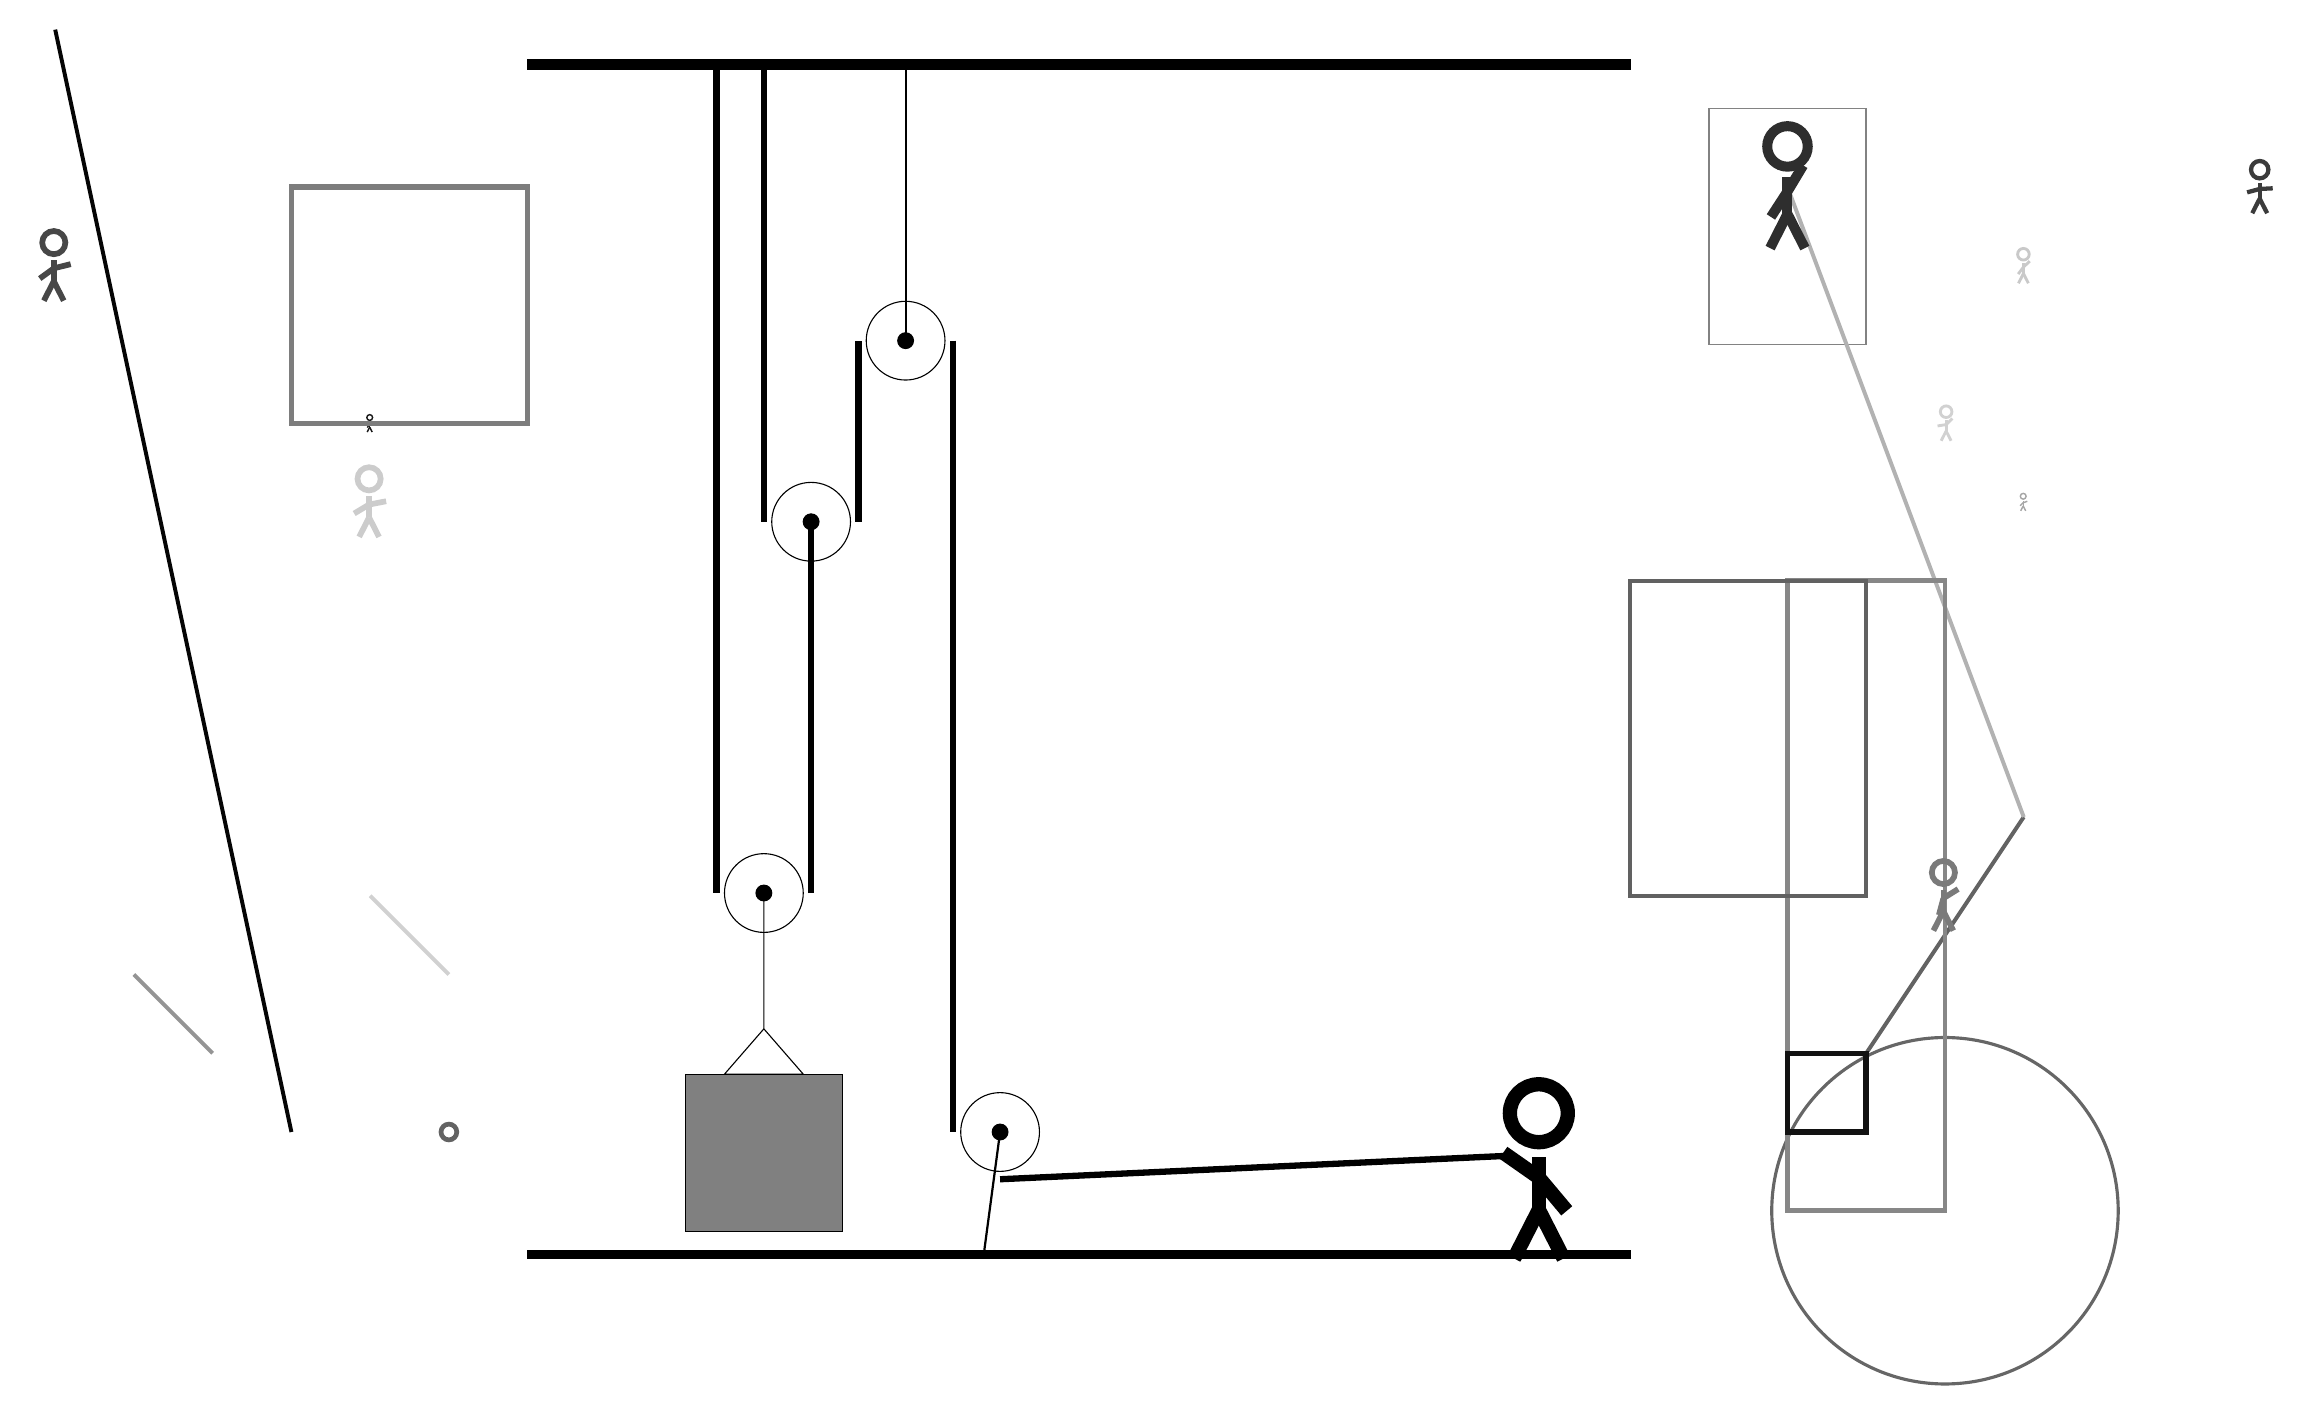
\begin{tikzpicture}
			%%%%% START %%%%%
			
			\draw[fill=black] (-2, 11.5) rectangle (12, 11.625);
			
			\draw (1, 1.035) circle (0.5);
			\draw[fill=black] (1, 1.035) circle (0.1);
			
			\draw (1.6, 5.75) circle (0.5);
			\draw[fill=black] (1.6, 5.75) circle (0.1);
			
			\draw (2.8, 8.05) circle (0.5);
			\draw[fill=black] (2.8, 8.05) circle (0.1);
			\draw[thick] (2.8, 8.05) -- (2.8, 11.5);
			
			\draw (4.0, -2) circle (0.5);
			\draw[fill=black] (4.0, -2) circle (0.1);
			\draw[thick] (4.0, -2) -- (3.8, -3.5);
			
			\draw (1, 1.035) -- (1, -0.69) -- (0.5, -1.265) -- (1.5, -1.265) -- (1, -0.69);
			\draw[fill=black!50] (0, -1.265) rectangle (2, -3.265);
			\draw[line width=0.8mm] (0.4, 11.5) -- (0.4, 1.035);
			\centerarc[line width=0.8mm](1, 1.035)(180:360:0.6);
			\draw[line width=0.8mm](1.6, 1.035) -- (1.6, 5.75);
			\draw[line width=0.8mm] (1.0, 11.5) -- (1.0, 5.75);
			\centerarc[line width=0.8mm](1.6, 5.75)(180:360:0.6);
			\draw[line width=0.8mm](2.2, 5.75) -- (2.2, 8.05);
			\centerarc[line width=0.8mm](2.8, 8.05)(0:180:0.6);
			\draw[line width=0.8mm] (3.4, 8.05) -- (3.4, -2);
			\centerarc[line width=0.8mm](4.0, -2)(0:90:-0.6);
			\draw[line width=0.8mm](4.0, -2.6) -- (10.5, -2.3);
			
			\draw[line width=0.2mm, color=black!49] (13, 8) rectangle (15, 11);
			
			\draw[line width=0.5mm, color=black!98](-5, -2) -- (-8, 12);
			\draw [line width=0.6mm, color=black!61](-3, -2) circle (0.1);
			\draw [line width=0.4mm, color=black!60](16, -3) circle (2.2);
			\draw[line width=0.5mm, color=black!18](-3, 0) -- (-4, 1);
			\node[line width=0.2mm, color=black!90] at (-4, 7) {\Strichmaxerl[1][56][29]};
			\node[line width=0.4mm, color=black!20] at (-4, 6) {\Strichmaxerl[4][31][11]};
			
			\draw[line width=0.5mm, color=black!61](15, -1) -- (17, 2);
			\node[line width=0.7mm, color=black!35] at (17, 6) {\Strichmaxerl[1][44][19]};
			
			\node[line width=0.7mm, color=black!77] at (20, 10) {\Strichmaxerl[3][15][3]};
			
			\draw[line width=0.5mm, color=black!30](14, 10) -- (17, 2);
			
			\node[line width=0.2mm, color=black!72] at (-8, 9) {\Strichmaxerl[4][36][14]};
			\draw[line width=0.6mm, color=black!47] (14, 5) rectangle (16, -3);
			
			\draw[line width=0.5mm, color=black!62] (12, 5) rectangle (15, 1);
			\node[line width=0.6mm, color=black!21] at (17, 9) {\Strichmaxerl[2][53][43]};
			\node[line width=0.3mm, color=black!82] at (14, 10) {\Strichmaxerl[7][57][59]};
			\draw[line width=0.7mm, color=black!51] (-2, 7) rectangle (-5, 10);
			\node[line width=0.7mm, color=black!18] at (16, 7) {\Strichmaxerl[2][9][44]};
			\draw[line width=0.7mm, color=black!93] (14, -2) rectangle (15, -1);
			
			\node[line width=0.6mm, color=black!52] at (16, 1) {\Strichmaxerl[4][75][32]};
			\draw[line width=0.5mm, color=black!42](-7, 0) -- (-6, -1);
			
			
			\node at (10.8, -2.5) {\Strichmaxerl[10][-35][-50]};
			
			\draw[fill=black] (-2, -3.5) rectangle (12, -3.6);
			
			%%%%% END %%%%%
		\end{tikzpicture}
	\end{figure}	
\end{document}